% MASc & PhD Thesis Template

% Department of Electrical & Computer Engineering (ECE)
% Queen's University 

% Requisitioned By: Professor Michael Greenspan
% Prepared By: Ian Maquignaz M.Eng, MASc

% Template Version 2.0 - September 2017\9

% >>> OPEN THIS FILE IN TeXstudio TO START WRITTING YOUR THESIS! <<< %
% Though Note! You should not need to edit this file (asside from section "0.2 - TITLE PAGE"). Edit the individual files that are loaded. 
% For example, where you see \prefacesection{Abstract}

% INSERT YOUR ABSTRACT %
In this works we describe a novel Thesis Template, to be used by students in Electrical \& Computer Engineering at Queen's University. This section entails the abstract of the document. , this loads your abstract from the file at Thesis/3_Preface/0_Preface/0_Abstract.tex. Open the file 0_Abstract.tex and edit.

% -> FILE DESCRIPTION :: Thesis.tex
%	This is the master file for your thesis Tex project and will combine all of the files toghether to create your thesis (Thesis.pdf). 

%	Thesis.tex will perform the followign actions:
%	 1) Import all the supplemental packages
%	 2) Set the styling for the document
%	 3) Combine the various chapters, sections and other components of your thesis into one document.
%	 4) Create LaTex generated sections, such as Table of Contex, Gloassary, and Bibliography  

%*************************************************************************************************************
% 0.0 - PREAMBLE - DO NOT MODIFY
%*************************************************************************************************************
% File containing packages to include. 
% --> Imports packages using \usepackage and sets basic configuration)
% MASc & PhD Thesis Template

% Department of Electrical & Computer Engineering (ECE)
% Queen's University 

% Requisitioned By: Professor Michael Greenspan
% Prepared By: Ian Maquignaz M.Eng, MASc

% Template Version 1.0 - September 2017

% -> FILE DESCRIPTION :: Preable.tex
%	This files defines the imports necessary for proper compiling of the thesis document and create the styling of the document.

% Created in 2003 By Michelle L. Crane, Queen's University
% Updated in 2011 By Andrew W L Dickinson, Queen's University
% Updated in 2013 By Kevin Hughes, Queen's University
% Updated in 2017 By Ian Maquignaz, Queen's University

%*************************************************************************************************************
% DOCUMENT
%*************************************************************************************************************
% -> This section defines the basic thesis document. 

% Set Document Type
\documentclass[12pt]{report}  

% Select Queen's University Thesis Package
\usepackage{0_Config/1_Styles/Queens_ECE_Thesis_Style}   
    
%*************************************************************************************************************
% PATCHING
%*************************************************************************************************************
% -> This section imports functionality which fixes Latex bugs

\usepackage{morewrites}
%\usepackage{scrwfile}

%*************************************************************************************************************
% SPACING
%*************************************************************************************************************
% -> This section defines the basic spacing options for the thesis document. 

\usepackage{indentfirst} % Indent first paragraph after header

%*******************************************************************************
% HEADINGS
%*******************************************************************************
% -> This changes the headings go that they are prettier, this can be commented out for traditional headings.

\usepackage{sectsty}

%*************************************************************************************************************
% FONTS
%*************************************************************************************************************
% -> This section defines the fonts for various document entities.

\allsectionsfont{\bfseries}% set all the section font to bfseries
\chapterfont{\centering\Large} % set the sizes of chapters, sections ...
\sectionfont{\normalsize}
\subsectionfont{\normalsize}

%*************************************************************************************************************
% FORMATING
%*************************************************************************************************************
% -> This section defines formatting Table of Contents entr
% example: Chapter 1 Introduction

\usepackage[subfigure]{tocloft}
\usepackage{tocloft}
\usepackage{multicol}

\renewcommand{\cftchappresnum}{Chapter }
\renewcommand{\cftchapaftersnum}{:}
\renewcommand{\cftchapnumwidth}{7em}

% for formatting Table of Contents entry for Appendix, example: Appendix 1: Stuff
\newcommand*\updatechaptername{%
   \addtocontents{toc}{\protect\renewcommand*\protect\cftchappresnum{Appendix }}
}

%*******************************************************************************
% FOOTNOTES
%*******************************************************************************
% -> This section defines formating for footnotes

\interfootnotelinepenalty=10000 % This line stops footnotes from splitting onto two pages.

%*******************************************************************************
% VERBATIM
%*******************************************************************************
% -> 

\usepackage{moreverb}        % Using this package to get better control of the
                             % verbatim environment, mostly for the use of the
                             % listing environment which puts line number
                             % beside each line.  Note that there has to be a number
                             % in each set of brackets, i.e., \begin{listing}[1]{1}.
                             % PDF info file is "The moreverb package" by
                             % Robin Fairbairns (rf@cl.cam.ac.uk) after
                             % Angus Duggan, Rainer Schopf and Victor Eijkhout, 2000/06/29.
%-------------------------------------------------------------------------------
%\usepackage{verbatim}        % allows the use of \begin{comment} and \end{comment}
                             % as well as \verbatiminput{file}
                             % Note:  when using verbatim to input from a text file,
                             % such as a specification or code, use \begin{singlespacing}
                             % and \end{singlespacing}.  Also, tabs are not read
                             % properly, so the input file must only use spaces.

%                             \begin{comment}
%                             Can also use the verbatim package for
%                             comments like this...
%                             \end{comment}


%*******************************************************************************
% GLOSSARY
%*******************************************************************************
% -> Creates the glossary

\usepackage[acronym,automake,toc]{glossaries}
\newglossary[slg]{symbol}{sym}{sdn}{List of Symbols}
\makeglossaries

% See Glossary/Glossary.tex for the content of your glossary

%*******************************************************************************
% INDEX
%*******************************************************************************
% -> Creates the Index

\usepackage{makeidx}         
\makeindex

%*******************************************************************************
% MATH
%*******************************************************************************
% -> Import and configure packages for math
\usepackage{mathrsfs}		 % For Symbols
\usepackage{amssymb}		 % For More Symbols
\usepackage{amsfonts}		 % For Other Symbols
\usepackage{amsmath}         % For Equations
\usepackage{amsthm}          % For Theorems & Definitions


% Using the amsthm package, define a new theorem environment for my
% definition.  * means don't number it.
\newtheorem*{definition}{Definition}
\usepackage{cases}           % to make numbered cases (equations)
\usepackage{calc}            % Used with the Ventry environment defined below.

%*******************************************************************************
% FLOATS, PLOTS, AND FIGURES
%*******************************************************************************
% -> This section defines and configures packages for various styles of floating objects and figures. 
 
\usepackage{graphicx}       % for graphic images (use \includegraphics[...]{file.eps})
%\usepackage{subfigure}      % for subfigures (figures within figures)
\usepackage{subfig}			% for subfigures (figures within figures). Same as subfigures except it works.
\usepackage{wrapfig}		% for wrapping text around figures
%\usepackage{boxedminipage}  % to make boxed minipages, i.e., boxes around figures
\usepackage{rotate}         % for use of \begin{sideways} and \end{sideways}
\usepackage{listings}       % for use of printing code blocks
\usepackage{pgfplots}		% for plots
\usepackage{pdfpages}		% for importing PDFs

% Define how the ``listings'' to look.
%\lstset{basicstyle=\footnotesize,, numbers=left, numberstyle=\small, stepnumber=1, numbersep=5pt, showspaces=false, lineskip=-1pt}

\usepackage{float}           % Using this package to get better control of floats
                             % including the ability to define new float types for
                             % specification and code listings.
                             % DVI info file is "An Improved Environment for Floats"
                             % by Anselm Lingnau, lingnau@tm.informatik.uni=frankfurt.de
                             % 1995/03/29.

% Style of float used for code listings
\floatstyle{ruled}
\newfloat{Listing}{H}{lis}[chapter]

                             % Note:  The listings don't have space between the chapters, unlike
                             % the standard list of tables etc.  At the end, copy the spacing
                             % commands from the .toc file and insert into the .lis file.  Then,
                             % DO NOT LATEX it again, simply go to the DVI viewer!

\usepackage{placeins} % for \FloatBarrier which stops floats from crossing a point

%*******************************************************************************
% TABLES
%*******************************************************************************
% -> This section defines tables

\usepackage{tabularx}        % Package used to make variable width-columns, i.e.,
                             % column widths are changed to fit the maximum width
                             % and text is wrapped nicely.

\usepackage{threeparttable}

\usepackage{lscape}			% For landscape
\usepackage{adjustbox}		% To adjust table width
\usepackage{multirow}		% For merging and splitting table cells

%*******************************************************************************
% CAPTIONS
%*******************************************************************************
% ->  This section defines captions

\usepackage{caption}   % Package used to make my captions 'hang', i.e., wrap around, but not under the name of the caption.
%\usepackage[justification=centering]{caption} % Captions that are centered
                             

% Find that the captions are too far from my verbatim figures, but if
% I change it to 0, then the captions are too close for my other types
% of figures.  Maybe set each one separately?
%\setlength{\abovecaptionskip}{1ex}

%\setlength{\textfloatsep}{1ex plus1pt minus1pt}

%\setlength{\intextsep}{1ex plus1pt minus1pt}

%\setlength{\floatsep}{1ex plus1pt minus1pt}

%*******************************************************************************
% MISCELLANEOUS
%*******************************************************************************
% ->  This section defines miscellaneous packages that facilitate miscelaneous things

\usepackage{layout}          % useful for determining the margins of a document
                             % use with \layout command
                             
\usepackage{changebar}       % Way of indicating modifications by putting bars in the
                             % margin.  Read about it in "The Latex Companion".
                             
\usepackage{enumitem}		% For enumerated lists

%*******************************************************************************
% REFERENCES ETC.
%*******************************************************************************
% ->  This section defines the reference section

\usepackage{varioref}        % Better page references, e.g., "on preceding page", etc.
                             % \vref{key} Create an enhanced reference.
                             % \vpageref[text]{key} Create an enhanced page reference.
                             % \vrefrange{key}{key} Create an enhanced range of references.
                             % \vpagerefrange[text]{key}{key} Create an enhanced range of page references.
                             % Note: doesn't really work for consecutive pages.

% Renewing the text for before and after
\renewcommand{\reftextafter}{on the next page}
\renewcommand{\reftextbefore}{on the previous page}
\usepackage{url}             % for use of \url - pretty web addresses
\usepackage{fancyhdr}
\usepackage{cite}

%*******************************************************************************
% Block Diagrams
%*******************************************************************************
% ->  This section defines imports for block diagrams and flow charts

\usepackage{tikz}
\usetikzlibrary{arrows,automata,arrows.meta}

% Block Diagram
\tikzstyle{block} = [draw,fill=blue!20,minimum size=2em]
\def\radius{.7mm} 
\tikzstyle{branch}=[fill,shape=circle,minimum size=3pt,inner sep=0pt]

% Flow Charts
\usepackage{pgf}
\usepackage[utf8x]{inputenc}
\usetikzlibrary{positioning,calc}
\tikzset{
	state/.style={
		rectangle,
		rounded corners,
		draw=black, very thick,
		minimum height=2em,
		inner sep=2pt,
		text centered,
	},
}

%*******************************************************************************
% HYPERLINKS (must be last)
%*******************************************************************************
% ->  This section defines how hyperlinks function

% Uncomment these next two lines for linkback to citation pages in biblio
% \renewcommand*\backref[1]{\ifx#1\relax \else \linebreak Cited on page(s): #1. \fi}

\hypersetup{
	colorlinks=true,  % Change links to being coloured text, no boxes
	linkcolor=blue,
	urlcolor=blue,
}
% Neat package to turn href, ref, cite, gloss entries
% into hyperlinks in the dvi file.
% Make sure this is the last package loaded.
% Use with dvips option to get hyperlinks to work in ps and pdf
% files.  Unfortunately, then they don't work in the dvi file!
% Use without the dvips option to get the links to work in the dvi file.

% Note:  \floatstyle{ruled} don't work properly; so change to plain.
% Not as pretty, but functional...
% The bookmarks option sets up proper bookmarks in the pdf file :)

% Need this command to allow hyperref to play nicely with gloss; otherwise
% almost every \gloss will cause an error...
%\renewcommand{\glosslinkborder}{0 0 0}

%*************************************************************************************************************
% 0.1 - DOCUMENT - DO NOT MODIFY
%*************************************************************************************************************
\begin{document}

%*************************************************************************************************************
% 0.2 - TITLE PAGE 
%*************************************************************************************************************
%	INSERT THE DETAILS OF YOUR THESIS
%	REMOVE THE '%' TO UNCOMMENT LINE

%\title{The Title Of Your Thesis}
%\author{Your Name}
%\supervisor{Supervisor's Name}
%\dept{Electrical And Computer Engineering}
%\degree{Your Degree Name}
%\copyrightyear{2017}

\beforepreface

%*******************************************************************************
% 0.3 - ABSTRACT
%*******************************************************************************
\prefacesection{Abstract}

% INSERT YOUR ABSTRACT %
In this works we describe a novel Thesis Template, to be used by students in Electrical \& Computer Engineering at Queen's University. This section entails the abstract of the document.    

%*******************************************************************************
% 0.4 - ACKNOWLEDGEMENTS
%*******************************************************************************
\phantomsection
\prefacesection{Acknowledgments}

% INSERT YOUR ACKNOWLEDGEMENTS %
I would like to acknowledge my parents and friends. This thesis, a manifestation of the many sleepless nights, would not have been possible without their support. This section highlights your acknowledgment of individuals whom you believe deserve recognition for their contribution towards making your achievement possible.  

\clearpage % keep this for proper page numbering!   

%*******************************************************************************
% 0.5 - STATEMENT OF ORIGINALITY - (Required for PhD only)
%*******************************************************************************
\phantomsection
\prefacesection{Statement Of Originality}

% INSERT STATEMENT OF ORIGINALITY (if required) %
The following works is my own and I hereby certify the intellectual content of this thesis is the product of my own work. All references and contributions of other individuals has been cited and sourced appropriately, as defined by the IEEE Citation Reference manual.\\[0.3in]

[This section is your statement of originality. The requirement differs for MASc and PhD, therefore it is recommended your discuss this section with your supervisor] 

   

%*******************************************************************************
% 0.6.1 - Table of Contents
%*******************************************************************************
% Print the Table of Contents 
\PageContentstrue

% To disable, use the following:
%\PageContentsfalse

%*******************************************************************************
% 0.6.2 - List of Tables
%*******************************************************************************
% Print the List of Tables
\PageTablestrue

% To disable, use the following:
%\PageTablesfalse

%*******************************************************************************
% 0.6.3 - List of Figures
%*******************************************************************************
% Print the List of Figures
\PageFigurestrue

% To disable, use the following:
%\PageFiguresfalse


%*******************************************************************************
% 0.6.4 - List of Code Snippets
%*******************************************************************************
% Print the List of Code Snippets
\PageCodeSnippetstrue

% To disable, use the following:
%\PageCodeSnippetsfalse

%*******************************************************************************
% 0.6.5 - List of Equations
%*******************************************************************************
% Print a list of all equations
\PageEquationstrue

% To disable, use the following:
%\PageEquationsfalse

%*******************************************************************************
% 0.6.6 - Glossary
%*******************************************************************************
% The Glossary 
\PageGlossariestrue

% To disable, use the following:
%\PageGlossariesfalse

% Include Glossary
% -> FILE DESCRIPTION :: Glossary.tex
%	This files contains all of your glossaries. It has been configured to have your main glossary (definitions), acronym glossary and symbols glossary.

% ---------------------------------------------------------------------------------------------%

% MAIN (Definitions) GLOSSARY
% \newglossaryentry{NameInLink}{
%	name={NameToShow},
%	sort=NameInSort,
%	description={What does it mean?}
%	}

\newglossaryentry{diction}
{
	name={diction},
	sort=diction,
	description={the choice and use of words and phrases in speech or writing}
}
\newglossaryentry{lexicon}
{
	name={lexicon},
	sort=lexicon,
	description={the vocabulary of a person, language, or branch of knowledge}
}

\newglossaryentry{prose}
{
	name={prose},
	sort=prose,
	description={written or spoken language in its ordinary form, without metrical structure}
}

% ---------------------------------------------------------------------------------------------%

% ACRONYMS
% \newacronym{NameInSort}{NameToShow}{Definition}
\newacronym{lol}{LOL!}{Laugh Out Loud}


% ---------------------------------------------------------------------------------------------%

% SYMBOLS
% \newglossaryentry{NameInLink}{
%	type=symbol, 
%	name={NameToShow},
%	sort=NameInSort,
%	description={What does it mean?}
%	}

\newglossaryentry{mySymbol}{
	type=symbol,
	name={\textrm{$\Upsilon$}},
	sort=thresh,
	description={Arbitrary symbol.}
}



% This line forces all entries into glossary, even if they have not been referenced
% UNCOMMENT THIS LINE TO INCLUDE ALL GLOSSARY ITEMS (Not just those referenced)
%\glsaddall

% UNCOMMENT INDIVIDUAL GLOSSARIES TO BE PRINTED (IF not using \PageGlossariestrue) %
%\printglossaries % Prints ALL glossaries.
%\printglossary % Print the terms glossary
%\printglossary[title = Glossary of Terms] % Print the terms glossary
%\printglossary[type=symbol, title=Glossary of Symbols] % Prints the acronym glossary
%\printglossary[type=\acronymtype,title=Glossary of Abbreviations] % Prints the abbreviation glossary

%*******************************************************************************
% 0.6.x - Apply Apply After Preface - DO NOT MODIFY
%*******************************************************************************
% Create afterpreface sections
\afterpreface


%*******************************************************************************
% 0.7 - CHAPTERS
%*******************************************************************************
% Include Chapters. Chapters are kept separated to make editing easier.
\singlespacing \doublespacing

% Chapter 1 - Introduction

\glsresetall % reset the glossary to expand acronyms again
\chapter[Introduction]{Introduction}\label{ch:Introduction}
\index{Introduction}

% Introduction
\section{Introduction}
\singlespacing
\begin{itemize}
	\item{What will this thesis demonstrate?}
\end{itemize}
\doublespacing

% Motivation
\section{Motivation}
\singlespacing
\begin{itemize}
	\item{What is the motivation to research this subject?}
	\item{What impact will your research have on the industry or the world?}
\end{itemize}
\doublespacing

The goal of this thesis is to demonstrate a novel methodology, a new generation of technology or an innovative system.  

% Problem Overview
\section{Problem Statement}
\singlespacing
\begin{itemize}
	\item{Existing Technology}
	\item{Limitations of existing technology}
\end{itemize}
\doublespacing

% Thesis Contributions
\section[Contributions]{Thesis Contributions}
The main contributions of this thesis are as follows:
\singlespacing
\begin{itemize}
	\item{We propose a novel methodology for solving a complex problem.}
	\item{We have greatly innovated on existing methodologies by using a new technique of our own conception}
	\item{We have formulated a new technique which we hope will be the inception of a new generation of technology}
\end{itemize}
\doublespacing


% Thesis Outline
\section[Outline]{Thesis Outline}
The remainder of this thesis is organized as follows:
\noindent\textbf{Chapter 2, Background:} Background\\
\noindent\textbf{Chapter 3, Methods:} Methodology\\
\noindent\textbf{Chapter 4, Results:} Experimental Results\\
\noindent\textbf{Chapter 5, Future Work And Conclusions:} Conclusion
% Chapter 2 - Background

\glsresetall % reset the glossary to expand acronyms again
\chapter[Background]{Background}\label{ch:Background}
\index{Background}

% Background
\section{Background}
\begin{itemize}
	\item{Broad description of subject}
	\item{Some relevant history}
	\item{Current implementations in industry}
	\item{New \& Related Research on the subject}
\end{itemize}

Citations can be included in your manuscript by referencing them. For example, if I wanted to cite XKCD for a comic (as I have in figure \ref{fig:DEFENCE}), I would just do \cite{xkcdThesis}.

%\subsection{Short name for the top of the page}{Long subsection title to start subsection}
\subsection[Glossaries]{Glossaries of Terms and Acronyms}

Latex allows you to add words and acronyms to a glossary which is found in \textit{2\_Glossaries/Glossary}. This feature benefits the reader, for when you use strong \gls{diction} in your \gls{lexicon}, the reader can click the hyperlink and see the definition to thus better understand your \gls{prose}.

The glossary also allows you to keep track of acronyms and symbols. In the case of acronyms, LaTex defines the acronym on first use (such as \gls{lol}), then use the acronym afterwards (\gls{lol}). 
\glsresetall % reset the glossary to expand acronyms again
Everything is hyperlinked to the glossary page of your thesis, and if you want, you can reset the glossary at any point to make the full definition of an acronym appear again using \textbackslash glsresetall (\gls{lol}). Symbols are not very interesting, but work like this: \gls{mySymbol}. Note the definition is not printed alongside the symbol.

\textbf{Glossaries, Bibliography or Index not showing up?}
Did you compile them? They are not automatic. You have to manually click \lq Bibliography\rq, \lq Glossary\rq, and \lq index\rq under the TeXstudio \textit{Tools} drop-down menu. 
% Chapter 3 - Methodology
% With Sample Figures From Kevin Hughes

\glsresetall % reset the glossary to expand acronyms again
\chapter[Methodology]{Methodology}\label{ch:Methodology}
\index{Methodology}

% Equations Sets Counter
% Needed for keeping track of Equations Sets! Include this at the top of each chapter
\newcounter{EquationCounter}[chapter]
\numberwithin{EquationCounter}{chapter}
\numberwithin{equation}{EquationCounter}

% Methodology
\section{Your Proposed Method}
\begin{itemize}
	\item{How does you research work?}
\end{itemize}

\section[Examples]{Examples of things}

\subsection{Tables}
Table \ref{tab:testTable} is an example of a table:

% Example Table
% I recommend using http://truben.no/latex/table/ to help with making tables
% reference in the text using \ref{tab.testTable}
\begin{table}[!htbp]
	\centering
	\caption{Test Table}
	\begin{tabular}{|l|l|l|} % options are l,c,r (left, center, right)
		\hline
		Things & Other Things & Last Thing \\
		\hline
		X & ~ & ~ \\
		\hline
		~ & X & ~ \\
		\hline
		~ & ~ & X \\
		\hline
	\end{tabular}
	\label{tab:testTable}
\end{table}

\clearpage

The following is an example of a flow diagram:  

% Sample Flow Diagram
\begin{figure}[h]
	\centering
	
	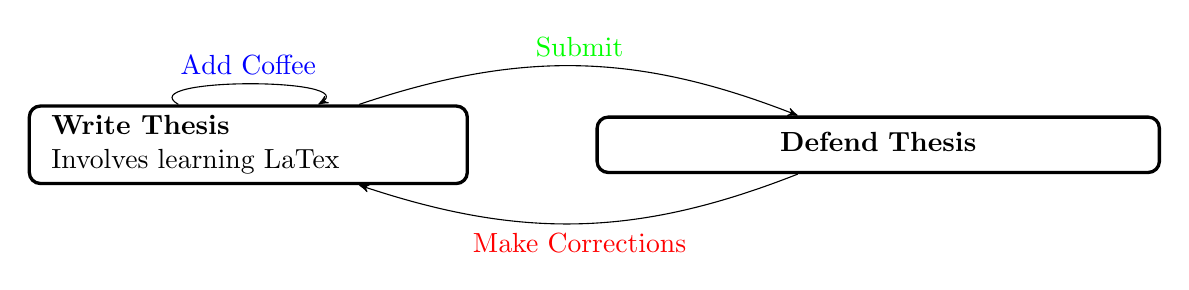
\begin{tikzpicture}[->,>=stealth']
	
	% Position of INPUT
	% Use previously defined 'state' as layout (see preamble)
	% use tabular for content to get columns/rows
	% parbox to limit width of the listing
	\node[state] (INPUT) 
	{
		\begin{tabular}{l}
		\textbf{Write Thesis}\\
		\parbox{5cm}
		{
			Involves learning LaTex
		}
		\end{tabular}
	};
	
	\node[state,    	% layout (defined above)
	text width=7cm, 	% max text width
	%	yshift=1cm, 		% move cm y
	xshift=7cm,
	right of=INPUT,
	%node distance=4cm,
	anchor=center] (OUTPUT) 
	{
		\begin{tabular}{l}
		\textbf{Defend Thesis}\\
		\end{tabular}
	};
	
	% draw the paths and and print some Text below/above the graph
	\path 
	(INPUT) 	edge[bend left=20]		node[anchor=south,above]{\textcolor{green}{Submit}}	(OUTPUT)
	(OUTPUT) 	edge[bend left=20]		node[anchor=south,below]{\textcolor{red}{Make Corrections}}	(INPUT)
	; % END PATH
	
	\draw 
	(INPUT) to [out=150,in=30] 	node[above,midway]{\textcolor{blue}{Add Coffee}} (INPUT)
	; % END DRAW
	
	\end{tikzpicture}
	\caption{A sample flow diagram} 
	\label{fig:SampleFlowDiagram}
\end{figure}


NOTE! The syntax for figures is:
\begin{center}
{\textbackslash}begin\{figure\}[placement specifier]\\
	... figure contents ...\\
{\textbackslash}end\{figure\}\\
\end{center}

See the wikibook on latex figures to see all the possibilities:\\
https://en.wikibooks.org/wiki/LaTeX/Floats,\_Figures\_and\_Captions\\

NOTE! There is an easier way to make diagrams than by coding them (as is demonstrated by the flow diagram below). See this website: https://www.draw.io/ will help you create an diagram easily. All you need to do is insert it in as a .jpg file (see the example insertion of a figure in \ref{fig:DEFENCE} (Appendix B)).

\clearpage
\subsection{Equations}

The following is an example of an equation:
\addtocounter{EquationCounter}{1} % Increment Equation Set counter
\setcounter{equation}{0} % Reset equation counter (equations inside set)
\begin{Equation}
	\begin{equation}
		\sqrt{\text{success}} = \text{effort}*\left(\frac{\text{time}+\text{coffee}}{\text{time}}\right)
		\label{eq:success}
	\end{equation}
	\begin{equation}
		\sqrt{\text{hydration}} = \text{water}-\left(\frac{\text{coffee}}{3}\right)
		\label{eq:water}
	\end{equation}
	\caption{This is a set of equations}
	\label{eqSet:coffeeWater}
\end{Equation}

Equation Set \ref{eqSet:coffeeWater} describes proper caffeine and hydration for successful thesis writting. Equation \ref{eq:success} demonstrates that the root of success is effort, enhanced by coffee intake and time. As such, coffee is an academic performance enhancing drug. Please abuse diligently and responsibly by consuming three cups of water per cup of coffee as shown in Equation \ref{eq:water}. This mitigates caffeine migraines as shown in Equation \ref{eq:waterIntake}.  

\begin{equation}
	\text{Result} = 
	\begin{cases}
	\text{hydration} \le 0 & \text{Bad!}\\
	1 \leq \text{hydration} \leq 6 & \text{Good!}\\
	\text{hydration} > 6 & \text{Overhydration, purge imminent.} \\
	\end{cases}
	\label{eq:waterIntake}
\end{equation}

The point of all this is to illustrate that equation sets (such as Equation Set \ref{eqSet:coffeeWater}) end up in the List of Equations, while basic equations (such as Equation \ref{eq:waterIntake}) do not. 

NOTE! For equations sets to work properly, don't forget to initialize the counter!! See the top of Methodology.tex for the three commands to apply at the top of each chapter.
% Chapter 4 - Experimental Results

\glsresetall % reset the glossary to expand acronyms again
\chapter[Results]{Experimental Results}\label{ch:Experimental Results}
\index{Experimental Results}

% Experimental Results
\section[Results]{Experimental Results}
\begin{itemize}
	\item{Describe the experimental setup (ie. Hardware)}
	\item{Describe your experiments}
	\item{Describe your results}
\end{itemize}


\clearpage

The following is an example code listing:

% Example By Kevin Hughes (see https://github.com/kevinhughes27/ThesisTemplate)

% Example Code Listing
% reference in the text using \ref{ls.testPlot}
\lstset{language=python}
\lstset{tabsize=4}
\lstset{commentstyle=\color{blue}}
\lstset{frame=single}
\lstset{label = ls.testPlot}
\lstset{caption = Test Plot Code }
\lstinputlisting[float=!htbp]{3_Chapters/4_Chapter_ExperimentalResults/Figures/SampleCode.py}{\tiny }


% Chapter 5 - Conclusion

\glsresetall % reset the glossary to expand acronyms again
\chapter[Conclusion]{Conclusion}\label{ch:Conclusion}
\index{Conclusion}

% Future Work
\section{Future Work}
\begin{itemize}
	\item{How do you hope to continue work on this topic?}
	\item{Are there possible extensions?}
	\item{What are some improvements that could be made?}
\end{itemize}

% Conclusion
\section{Conclusion}
\begin{itemize}
	\item{Restate the problem. State the novel solution.}
	\item{Summarize what has been accomplished}
	\item{Summarize any limitations}
	\item{What worked really well and has a big impact?}
\end{itemize}

%*******************************************************************************
% 0.8 - BIBLIOGRAPHY
%*******************************************************************************

% Put in \nocite{*} so all entries in the bibliography are included
\nocite{*}

% Print Bibliogrpahy
\phantomsection

% Uncomment for a plain bibliography else use IEEE style below
%\bibliographystyle{plain}
%\bibliography{4_References/References}

% IEEE Bibliography
\bibliographystyle{IEEEtran}
\bibliography{IEEEabrv,4_References/References}

\clearpage

%*******************************************************************************
% 0.9.1 - APPENDICES
%*******************************************************************************
\updatechaptername
\appendix

% Appendix A
\chapter{Supporting Data}

Appendix sections are where you can place large figures, data tables, and spinets of code. Use appendices to your benefit to keep the body of your thesis concise!\\

The lyrics found below are for your enjoyment, but also serve an important role in demonstrating latex syntax for formating text and in-text citations.  

\section{Lyrics to Soft Kitty}

\begin{center}
\mbox{}\\[0.2in]
Soft kitty, warm kitty\\
Little ball of fur\\
Happy kitty, sleepy kitty\\
Purr, purr, purr\\[0.5in]


This has been brought to you by Sheldon Cooper \cite{BigBang}
\end{center}

\clearpage

% Appendix B
\chapter{Satirical Support}

This section provides some comic relief. In addition, it serves as an example of how to insert an image into your thesis with proper caption, label and citation.

\section[XKCD]{Advice from XKCD:}
	\begin{figure}[h]
		\centering
		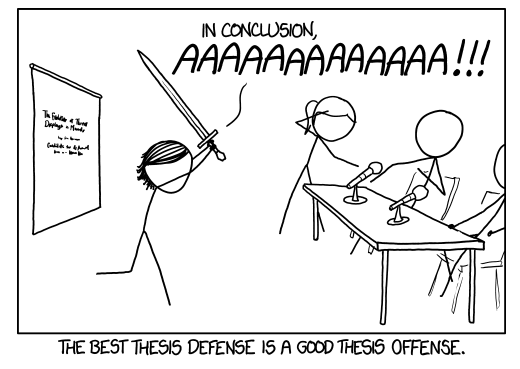
\includegraphics[width = 4.5in]{5_Appendices/Appendix_B/Figures/Thesis_Defence.png}
		\caption{You must prepare to defend your thesis \cite{xkcdThesis}} 
		\label{fig:DEFENCE}
	\end{figure}
\clearpage

%*******************************************************************************
% 0.9.2 - INDEX
%*******************************************************************************
% Creates the index
% Uncomment if an INDEX should be created

\printindex


%*************************************************************************************************************
% 1.0 - END OF DOCUMENT
%*************************************************************************************************************
\end{document}
